\section*{Objectives}
\begin{outline}
    \1 Wrap up SVM
    \1 Using $f(\alpha)$ to optimize
        \2 If optimized, we know $w$ and $b$
    \1 Try optimizing using \textbf{direct method}, but this will present an issue
    \1 Try optimizing with \textbf{indirect methods} using gradient descent based methods
    \1 Try optimizing with \textbf{backpropagation}
        \2 Backpropagation is the crux of DL (deep learning)
        \2 Deep learning provides a solution for non-linear data 

\end{outline}

\section*{Optimizing with $f(\alpha)$}

Continuing from the previous lecture, we have the equation:

\begin{equation}
f(\alpha) = \sum\limits_{i=1}^{n} \alpha_i - \frac{1}{2} \sum\limits_{i=1}^{n} \sum\limits_{j=1}^{n} \alpha_i \alpha_j y_i y_j x_i^T x_j
\end{equation}

The last term in this expression, $x_i^T x_j$, can be separated from the rest of the expression using \textbf{kernelization}. This process adds dimensionality that allows non-linearly separable data to be separated by a plane. For now, we will avoid using this method, but it's good to know.

\textbf{Kernelization} is a technique in SVM that uses kernel functions to transform data that can't be separated by a straight line into a higher dimensional space where a straight line can separate it.

Using purely algebra, we can simplify equation 1 a bit. Let's take a closer look at the second term in our equation. This is what it looks like if we have a vector with three components:

\[
\sum\limits_{i=1}^{3} \sum\limits_{j=1}^{3} \alpha_i \alpha_j y_i y_j x_i x_j = \alpha_1\alpha_1y_1y_1x_1x_1 + \alpha_1\alpha_2y_1y_2x_1x_2 + ... + \alpha_3\alpha_3y_3y_3x_3x_3
\]

Let's look at the Lagrange multipliers by themselves for this demonstration:

\[
\sum\limits_{i=1}^{3} \sum\limits_{j=1}^{3} \alpha_i \alpha_j y_i y_j x_i x_j = 
\begin{pmatrix}
\alpha_1\alpha_1 + \alpha_1\alpha_2 + \alpha_1\alpha_3 
\\
+ \alpha_2\alpha_1 + \alpha_2\alpha_2 + \alpha_2\alpha_3 
\\
+ \alpha_3\alpha_1 + \alpha_3\alpha_2 + \alpha_3\alpha_3
\end{pmatrix}
\]

Still using just algebra, we can rearrange and combine terms to rewrite each as $\alpha^2$. This pattern also applies to the $y$ and $x$ constants. Therefore, equation 1 can be rewritten as:

\begin{equation}
f(\alpha) = \sum\limits_{i=1}^{n} \alpha_i - \frac{1}{2} \sum\limits_{i=1}^{n} \alpha_i^2 y_i^2 x_i^T x_j
\end{equation}

Let's review a couple definitions before we continue. When we think of $\alpha$, we should think of it as a vector with components like such:

\[
\alpha = 
\begin{bmatrix} 
\alpha_1 \\ 
\alpha_2 \\ 
\vdots \\
\alpha_n
\end{bmatrix}
\]

where most components are equal to zero. With this definition, we can rewrite $f(\alpha)$:

\[
    f(\alpha) = f\begin{pmatrix}\begin{bmatrix} 
\alpha_1 \\ 
\alpha_2 \\ 
\vdots \\
\alpha_n
\end{bmatrix}\end{pmatrix}
\]

For some component in $\alpha$, let's call it $\alpha_k$, we can write $f(\alpha_k)$:

\begin{equation}
    f(\alpha_k) = \sum\limits_{i=1}^{n}\alpha_i - \frac{1}{2}\alpha_k^2 y_k^2 x_k^Tx_k - \alpha_k y_k \sum_{\substack{i=1 \\ i \ne k}}^n \alpha_i y_i x_i^Tx_k
\end{equation}

We do this reformatting because equation 3 will be easier to partially derive than equation 1. Now, our goal is to find $\nabla f'(\alpha) = \frac{\partial f}{\partial \alpha_k}$. Let's rewrite this equation to get something we can use. We are able to separate out a term with all of our variables with subscript $k$ because our summation specifies $i \ne k$ and jumps over $\alpha_k, y_k$ and $x_k$. Also, when we take the derivative of $\alpha^2$, we get $2\alpha$ which cancels out the factor of $\frac{1}{2}$:

\[
\nabla f(\alpha_k) = 1 - \alpha_ky_k^2x_k^Tx_k - y_k \sum_{\substack{i=1 \\ i \ne k}}^n \alpha_i y_i x_i^Tx_k
\]

We can take out a common factor of $y_k$:

\[
\nabla f(\alpha_k) = 1 - y_k [\sum\limits_{i=1}^{n} \alpha_iy_ix_i^Tx_k]
\]

Now, put $y_k$ back into our summation like so:

\[
\nabla f(\alpha_k) = 1 - \sum\limits_{i=1}^{n} \alpha_iy_iy_kx_i^Tx_k
\]

With this definition of $\nabla f(\alpha_k)$, we can rewrite this into vector format where $[1 - \sum\limits_{i=1}^{n} \alpha_iy_iy_kx_i^Tx_k]$ is the $k$th component in $\nabla f(\alpha)$. Then, to take a gradient descent, we set our equation equal to $\vec{0}$. Now we have: 

\begin{equation}
\nabla f(\alpha) = \begin{bmatrix}
        1 - \sum\limits_{i=1}^{n} \alpha_iy_iy_1x_i^Tx_1 \\
        \vdots \\
        1 - \sum\limits_{i=1}^{n} \alpha_iy_iy_kx_i^Tx_k \\
        \vdots \\
        1 - \sum\limits_{i=1}^{n} \alpha_iy_iy_nx_i^Tx_n \\
    \end{bmatrix} =
    \vec{0} = \begin{bmatrix}
    0\\
    0\\
    \vdots\\
    0
\end{bmatrix}
\end{equation}

Let's rework this slightly by adding the second term to all components in both vectors; this gives us:

\[
\nabla f(\alpha) = \begin{bmatrix}
        \sum\limits_{i=1}^{n} \alpha_iy_iy_1x_i^Tx_1 \\
        \vdots \\
        \sum\limits_{i=1}^{n} \alpha_iy_iy_nx_i^Tx_n \\
    \end{bmatrix} =
    \begin{bmatrix}
    1\\
    \vdots\\
    1
\end{bmatrix}
\]

Note that $x_i$ and $y_i$ are known, and $\alpha_i$ is not. We can rewrite these vectors as a matrix of known $x$ and $y$ values multiplied by $\vec{\alpha}$:

\begin{equation}
\begin{bmatrix} 
y_1 y_1 x_1^T x_1 & y_1 y_2 x_1^T x_2 & \dots & y_1 y_n x_1^T x_n \\
y_2 y_1 x_2^T x_1 & y_2 y_2 x_2^T x_2 & \dots & y_2 y_n x_2^T x_n \\
\vdots & \vdots & \ddots & \vdots \\
y_k y_1 x_k^T x_1 & \dots & \dots & y_k y_n x_k^T x_n\\
\vdots & \vdots & \ddots & \vdots \\
y_n y_1 x_n^T x_1 & y_n y_2 x_n^T x_2 & \dots & y_n y_n x_n^T x_n
\end{bmatrix}
    *
    \begin{bmatrix}
        \alpha_1\\
        \alpha_2\\
        \vdots\\
        \alpha_k\\
        \vdots\\
        \alpha_n
    \end{bmatrix} 
    = 
    \begin{bmatrix}
    1\\
    1\\
    \vdots\\
    1\\
    \vdots\\
    1
\end{bmatrix}
\end{equation}

where the first matrix is $n$ x $n$ and both vectors are $n$ x 1. When we do this matrix multiplication, we multiply each row by $\vec{\alpha}$. This is what we get when we multiply the first row of the matrix by $\vec{\alpha}$:

\[
\sum\limits_{i=1}^{n} y_1 y_i x_1 ^T x_i \cdot \alpha_i
\]

We can rewrite this abstractly as:

\[
Q \alpha = 1 \implies \alpha = Q^{-1} \cdot 1
\]

But here's our issue: we don't know what $Q$ is. Additionally, taking the inverse of a matrix is a difficult calculation that's in $O(n^3)$ and the results of such an operation are numerically unstable and untrustworthy. Therefore, this \textbf{direct solution} only works theoretically. Let's move on to try the \textbf{indirect} or \textbf{iterative method}.

\textbf{More on Matrices:} When you have a bloated matrix or a matrix that is poorly conditioned. Direct optimization can actually lead to numerical instability. This is important as it is not uncommon in real world data sets. 

The iterative method is defined by the \textbf{update rule}:

\begin{equation}
    \alpha_{new} = \alpha_{old} - \eta \nabla L (\alpha_{old})
\end{equation}

where $L$ is our loss function and $\eta$ is a hyper-parameter representing the learning rate, often set to $0.1$ or $0.01$. Recall that our goal is always to minimize loss for maximum accuracy. 

The second term, $[\eta \nabla L (\alpha_{old})]$, is subtracted from the equation because we want to step in the direction that will \textit{minimize} the loss function. Let's see an example of a convex quadratic loss function:

\begin{center}
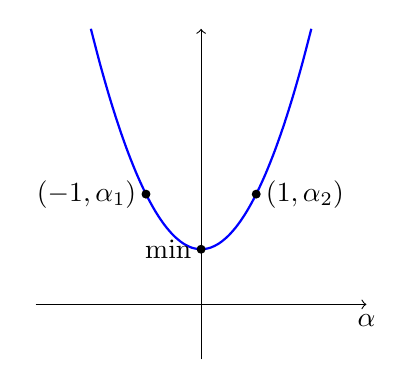
\begin{tikzpicture}[scale=0.7]
    % Draw the x-axis labeled as \alpha, moved up to y=2
    \draw[->] (-3,1) -- (3,1) node[anchor=north] {$\alpha$};
    % Draw the y-axis without a label
    \draw[->] (0,0) -- (0,6);

    % Plot the function x^2 with the new y-intercept position (+2)
    \draw[domain=-2:2, smooth, variable=\x, thick, blue] 
        plot ({\x}, {(\x)*(\x) + 2});
        
    % Add a node at the y-intercept (0,2)
    \filldraw[black] (0,2) circle (2pt) node[anchor=east] {min};
    \filldraw[black] (1,3) circle (2pt) node[anchor=west] {$(1, \alpha_2)$};
    \filldraw[black] (-1,3) circle (2pt) node[anchor=east] {$(-1, \alpha_1)$};
\end{tikzpicture}
\end{center}

The goal is to move closer to the function's minimum, marked clearly above, with each iteration of $\alpha_x$. The step size will decrease as we go because the gradient approaches $0$; we subtract less and less each step as our slope flattens. 

Above, we are working with vanilla gradient descent. This can work on a simple function like $x^2$; however, when we get more complex, wiggly functions, a simple gradient descent like vanilla can get stuck in local minimums.

To get around this, we can use a more robust gradient descent like ADAM. In the next lecture, we will learn more about using gradient descents. 
